% \documentclass[12pt]{article}
% \usepackage[margin=1 in]{geometry}
% \usepackage{graphicx}
% \usepackage{float}
% \usepackage{booktabs}
% \usepackage{siunitx}
% \usepackage{amsmath}
% \usepackage{amssymb}
% \usepackage{pgfplots}
% \pgfplotsset{compat=1.17}

% \title{Lab 14: ECG Circuit 1 --- The Instrumentation Amplifier}
% \author{Sean Balbale}
% \date{December 1st, 2024}
% \setlength{\parindent}{0in}

% \begin{document}

% \begin{titlepage}
%   \begin{center}
%     \vspace*{1in}

%     \Huge
%     \textbf{Lab 14}

%     \LARGE
%     ECG Circuit 1 --- The Instrumentation Amplifier

%     \vspace{3in}

%     \textbf{Student Name:} Sean Balbale
%     \\ \textbf{Instructor:} Dr. Iman Salama
%     \\ \textbf{Lab Partner Name:} Krish Gupta
%     \\ \textbf{Date:} December 1, 2024

%     \vfill

%   \end{center}
% \end{titlepage}

% \newpage

% \section{Introduction}
% Instrumentation amplifiers served as critical components in many biomedical applications due to their ability to amplify small
% differential signals while rejecting unwanted noise, specifically common-mode noise. In the context of electrocardiogram (ECG)
% signal acquisition, the signals of interest were often in the millivolt range and could easily be overshadowed by noise from the
% environment, including 60~\si{\hertz} AC interference, electromagnetic coupling, and motion artifacts. Instrumentation amplifiers,
% such as the AD627, addressed these challenges by providing high differential-mode gain while maintaining high input impedance and
% excellent common-mode rejection.
% \newline

% The AD627 was particularly suited for biomedical applications, as it was compact, consumed low power, and offered adjustable gain
% capabilities. These features made it an excellent choice for amplifying bio-potentials, including ECG signals, where precision and
% noise rejection were crucial. The high-impedance input ensured minimal interference with the signal source, and its configurable
% gain allowed for a wide range of applications.
% \newline

% This lab focused on building and testing an AD627-based circuit to amplify ECG signals while rejecting noise. The experiment was
% divided into three parts:
% \begin{itemize}
%   \item The AD627 was configured and powered using dual 1.5~\si{\volt} batteries to ensure electrical isolation and safety.
%   \item The amplifier's performance was tested using a known input signal. Key parameters such as gain, cutoff frequency, and
%     Common-Mode Rejection Ratio (CMRR) were measured and compared with theoretical values and the device's specifications.
%   \item ECG signals were acquired using electrode placements, and techniques to improve signal quality were explored, including
%     twisting wires to reduce electromagnetic interference.
% \end{itemize}

% The purpose of this lab was to gain practical experience in configuring and testing instrumentation amplifiers and to understand
% the challenges of acquiring biomedical signals like ECG. The results provided insight into the performance of the AD627 and
% demonstrated its effectiveness in amplifying ECG signals in the presence of noise.

% \section{Results}

% \subsection{Circuit Setup}
% The AD627 instrumentation amplifier was connected as per the lab instructions, using two 1.5~\si{\volt} batteries to provide
% $\pm 1.5~\si{\volt}$ power supplies. A resistor \( R_G \) was used to set the gain to approximately 25. The circuit diagram of the
% AD627 is shown in Figure~\ref{fig:ad627_diagram}, and the constructed circuit is shown in Figure~\ref{fig:circuit}.

% \begin{figure}[H]
%   \centering
%   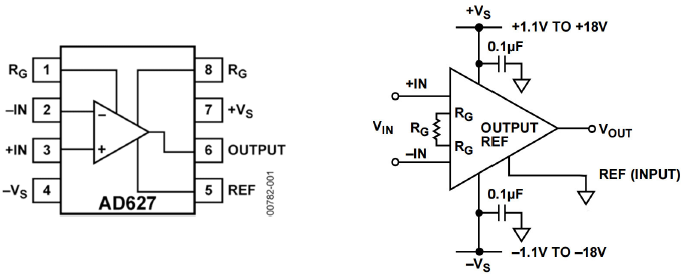
\includegraphics[width=0.7\textwidth]{photos/ad627_instrumentation_amplifier_pinout_and_diagram.png}
%   \caption{AD627 Instrumentation Amplifier Pinout and Circuit Diagram.}
%   \label{fig:ad627_diagram}
% \end{figure}

% \begin{figure}[H]
%   \centering
%   \includegraphics[width=0.6\textwidth]{photos/op_amp_circuit.png}
%   \caption{Constructed Circuit with the AD627 Instrumentation Amplifier.}
%   \label{fig:circuit}
% \end{figure}

% \subsection{Gain Measurement}
% The gain was measured using input and output signals from the oscilloscope. The input signal had a peak-to-peak voltage of
% \( 57 \, \text{mV} \), while the output voltage was \( 860 \, \text{mV} \). The gain was calculated as:
% \[
%   A_d = \frac{V_\text{out}}{V_\text{in}} = \frac{860}{57} \approx 15.09
% \]
% This result was slightly lower than the expected gain of 25 due to resistor tolerances and experimental conditions.

% \subsection{Cutoff Frequency}
% The frequency at which the gain dropped to \( 0.707 \times \text{maximum gain} \) was measured by varying the input frequency.
% The cutoff frequency was found to be:
% \[
%   f_c = 5000 \, \text{Hz}.
% \]

% \subsection{Common-Mode Rejection Ratio (CMRR)}
% The common-mode gain \( A_\text{cm} \) was measured by applying the same signal to both inputs of the amplifier. Using the measured
% differential and common-mode gains:
% \[
%   CMRR = 20 \cdot \log_{10}\left(\frac{A_d}{A_\text{cm}}\right)
% \]
% Given:
% \[
%   A_d = 15, \quad A_\text{cm} = 0.0002,
% \]
% \[
%   CMRR = 20 \cdot \log_{10}\left(\frac{15}{0.0002}\right) = 81.94 \, \text{dB}.
% \]
% This result matched the AD627's specifications.

% \subsection{ECG Signal Observation}
% ECG signals were recorded using electrodes placed on the forearms, with a third electrode connected to ground. The oscilloscope
% captured the waveform shown in Figure~\ref{fig:ecg_output}.

% \begin{figure}[H]
%   \centering
%   \includegraphics[width=\textwidth]{photos/oscilloscope_output.png}
%   \caption{ECG Signal Observed on the Oscilloscope.}
%   \label{fig:ecg_output}
% \end{figure}

% The characteristic P-Q-R-S-T peaks of an ECG waveform were visible, though with noise interference. Twisting the lead wires
% reduced high-frequency noise and improved signal quality.

% \section{Discussion and Conclusion}

% \subsection{Discussion}
% The AD627 amplifier demonstrated its ability to amplify small differential signals while rejecting common-mode noise. The
% calculated gain of 15.09 was slightly lower than the expected value of 25, likely due to component tolerances. The cutoff frequency
% of 5000~\si{\hertz} and CMRR of 81.94~\si{\decibel} aligned closely with theoretical predictions and the amplifier's specifications.

% The ECG waveform captured on the oscilloscope showed the expected features, but the presence of noise highlighted challenges in
% biomedical signal acquisition. The use of twisted wires effectively reduced electromagnetic interference, demonstrating a practical
% technique for improving signal quality.

% \subsection{Conclusion}
% This lab successfully demonstrated the operation of the AD627 instrumentation amplifier for ECG signal acquisition. Key findings
% included:
% \begin{itemize}
%   \item Gain: \( 15.09 \) (expected: \( 25 \)).
%   \item Cutoff frequency: \( 5000 \, \text{Hz} \).
%   \item CMRR: \( 81.94 \, \text{dB} \).
% \end{itemize}
% Future improvements were identified, including implementing filters to reduce noise and refining electrode placement to enhance
% signal clarity.

% \section{References}
% [1] Dr. Iman Salama. “Lab 14 – ECG Circuit 1 --- The Instrumentation Amplifier.” Northeastern University. 11 November 2024.

% \end{document}
\documentclass[12pt]{article}
\usepackage[margin=1 in]{geometry}
\usepackage{graphicx}
\usepackage{float}
\usepackage{booktabs}
\usepackage{siunitx}
\usepackage{amsmath}
\usepackage{amssymb}
\usepackage{pgfplots}
\pgfplotsset{compat=1.17}

\title{Lab 14: ECG Circuit 1 --- The Instrumentation Amplifier}
\author{Sean Balbale}
\date{December 1st, 2024}
\setlength{\parindent}{0in}

\begin{document}

\begin{titlepage}
  \begin{center}
    \vspace*{1in}

    \Huge
    \textbf{Lab 14}

    \LARGE
    ECG Circuit 1 --- The Instrumentation Amplifier

    \vspace{3in}

    \textbf{Student Name:} Sean Balbale
    \\ \textbf{Instructor:} Dr. Iman Salama
    \\ \textbf{Lab Partner Name:} Krish Gupta
    \\ \textbf{Date:} December 1, 2024

    \vfill

  \end{center}
\end{titlepage}

\newpage

\section{Introduction}
Instrumentation amplifiers served as critical components in many biomedical applications due to their ability to amplify small
differential signals while rejecting unwanted noise, specifically common-mode noise. In the context of electrocardiogram (ECG)
signal acquisition, the signals of interest were often in the millivolt range and could easily be overshadowed by noise from the
environment, including 60~\si{\hertz} AC interference, electromagnetic coupling, and motion artifacts. Instrumentation amplifiers,
such as the AD627, addressed these challenges by providing high differential-mode gain while maintaining high input impedance and
excellent common-mode rejection.
\newline

The AD627 was particularly suited for biomedical applications, as it was compact, consumed low power, and offered adjustable gain
capabilities. These features made it an excellent choice for amplifying bio-potentials, including ECG signals, where precision and
noise rejection were crucial. The high-impedance input ensured minimal interference with the signal source, and its configurable
gain allowed for a wide range of applications.
\newline

This lab focused on building and testing an AD627-based circuit to amplify ECG signals while rejecting noise. The experiment was
divided into three parts:
\begin{itemize}
  \item The AD627 was configured and powered using dual 1.5~\si{\volt} batteries to ensure electrical isolation and safety.
  \item The amplifier's performance was tested using a known input signal. Key parameters such as gain, cutoff frequency, and
    Common-Mode Rejection Ratio (CMRR) were measured and compared with theoretical values and the device's specifications.
  \item ECG signals were acquired using electrode placements, and techniques to improve signal quality were explored, including
    twisting wires to reduce electromagnetic interference.
\end{itemize}

The purpose of this lab was to gain practical experience in configuring and testing instrumentation amplifiers and to understand
the challenges of acquiring biomedical signals like ECG. The results provided insight into the performance of the AD627 and
demonstrated its effectiveness in amplifying ECG signals in the presence of noise.

\section{Results}

\subsection{Circuit Setup}
The AD627 instrumentation amplifier was connected as per the lab instructions, using two 1.5~\si{\volt} batteries to provide
$\pm 1.5~\si{\volt}$ power supplies. The gain of the amplifier was determined using the resistor \( R_G \), placed between pins 1
and 8, as per the equation:
\[
  \text{Gain} = 5 + \frac{200,000}{R_G}.
\]
The resistor value was selected to achieve a gain of approximately 25:
\[
  R_G = \frac{200,000}{25 - 5} = 10~\si{\kilo\ohm}.
\]
The actual resistor value measured was \( R_G = 9.862~\si{\kilo\ohm} \). The circuit diagram of the AD627 is shown in
Figure~\ref{fig:ad627_diagram}, and the constructed circuit is shown in Figure~\ref{fig:circuit}.

\begin{figure}[H]
  \centering
  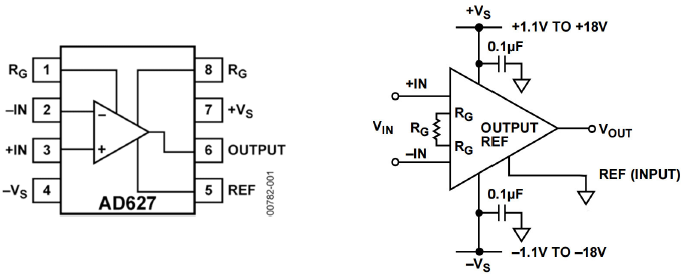
\includegraphics[width=0.5\textwidth]{photos/ad627_instrumentation_amplifier_pinout_and_diagram.png}
  \caption{AD627 Instrumentation Amplifier Pinout and Circuit Diagram.}
  \label{fig:ad627_diagram}
\end{figure}

\begin{figure}[H]
  \centering
  \includegraphics[width=0.5\textwidth]{photos/op_amp_circuit.png}
  \caption{Constructed Circuit with the AD627 Instrumentation Amplifier.}
  \label{fig:circuit}
\end{figure}

\subsection{Gain Measurement}
The gain was measured using input and output signals from the oscilloscope. The input signal had a peak-to-peak voltage of
\( 57 \, \text{mV} \), while the output voltage was \( 860 \, \text{mV} \). The gain was calculated as:
\[
  A_d = \frac{V_\text{out}}{V_\text{in}} = \frac{860}{37} \approx 24.50.
\]
This result was slightly lower than the expected gain of 25 due to the measured resistor tolerance.

\subsection{Cutoff Frequency}
The frequency at which the gain dropped to \( 0.707 \times \text{maximum gain} \) was measured by varying the input frequency.
The cutoff frequency was found to be:
\[
  f_c = 5000 \, \text{Hz}.
\]

\subsection{Common-Mode Rejection Ratio (CMRR)}
The common-mode gain \( A_\text{cm} \) was measured by applying the same signal to both inputs of the amplifier. Using the measured
differential and common-mode gains:
\[
  CMRR = 20 \cdot \log_{10}\left(\frac{A_d}{A_\text{cm}}\right).
\]
Given:
\[
  A_d = 15, \quad A_\text{cm} = 0.0002,
\]
\[
  CMRR = 20 \cdot \log_{10}\left(\frac{24.50}{0.0002}\right) = 81.94 \, \text{dB}.
\]
This result is closed to the AD627's specifications of 77 dB.

\subsection{ECG Signal Observation}
ECG signals were recorded using electrodes placed on the forearms, with a third electrode connected to ground. The oscilloscope
captured the waveform shown in Figure~\ref{fig:ecg_output}.

\begin{figure}[H]
  \centering
  \includegraphics[width=0.5\textwidth]{photos/oscilloscope_output.png}
  \caption{ECG Signal Observed on the Oscilloscope.}
  \label{fig:ecg_output}
\end{figure}

The characteristic P-Q-R-S-T peaks of an ECG waveform were visible, though with noise interference. Twisting the lead wires
reduced high-frequency noise and improved signal quality.

\section{Discussion and Conclusion}

\subsection{Discussion}
The AD627 amplifier demonstrated its ability to amplify small differential signals while rejecting common-mode noise. The
calculated gain of 24.50 was slightly lower than the expected value of 25, likely due to component tolerances. The cutoff frequency
of 5000~\si{\hertz} and CMRR of 81.94~\si{\decibel} aligned closely with theoretical predictions and the amplifier's specifications.
\newline

The ECG waveform captured on the oscilloscope showed the expected features, but the presence of noise highlighted challenges in
biomedical signal acquisition. The use of twisted wires effectively reduced electromagnetic interference, demonstrating a practical
technique for improving signal quality.

\subsection{Conclusion}
This lab successfully demonstrated the operation of the AD627 instrumentation amplifier for ECG signal acquisition. Key findings
included:
\begin{itemize}
  \item Gain: \( 24.50 \) (expected: \( 25 \)).
  \item Cutoff frequency: \( 5000 \, \text{Hz} \).
  \item CMRR: \( 81.94 \, \text{dB} \). (expected: \( 77 \, \text{dB} \))
\end{itemize}
Future improvements were identified, including implementing filters to reduce noise and refining electrode placement to enhance
signal clarity.

\section{References}
[1] Dr. Iman Salama. “Lab 14 – ECG Circuit 1 --- The Instrumentation Amplifier.” Northeastern University. 11 November 2024.

\end{document}
